\chapter{Verfahren zur Optimierung von Augmented Reality durch Tiefeninformationen}

Anhand der Klassifizierung von Project Tango bezüglich Augmented Reality aus Abschnitt \ref{sec:classification_project_tango}, kann bereits festgehalten werden, dass sich das Gerät, durch die Verfügbarkeit von intrinsischen und extrinsischen Kameraparametern, für den Einsatz von Augmented Reality gut eignet. Um jedoch eine für den Betrachter eine effektive und optimierte Augmented Reality Anwendung umsetzen zu können, benötigt man laut \citet{azuma2001recent} die Möglichkeit mehr Informationen über relevante Objekte im realen Raum zu ermitteln. Diese Informationen könnten zum Beispiel eine Tiefenüberdeckung von virtuellen Objekten durch reale Objekte ermöglichen, eine Interaktion mit realen Objekten durch die Anwendung von physikalischen Modellen und Kollisionen generieren oder die Funktion anhand semantischer Einordnung der Umgebung variieren. \\

Zur zuletzt erwähnte Kontextsensitivität existieren viele Ansätze, basierend auf optischen Merkmalen der Umgebung. So kann zum Beispiel ein optisches Tracking von realen Objekten, wie von \citet{lee2008hybrid} beschrieben, umgesetzt werden. Project Tango nutzt bereits optische Merkmale um \enquote{Motion Tracking} und \enquote{Area Learning} umzusetzen. Wären diese Merkmale für den Nutzer als Schnittstelle verfügbar, könnte man mit Diesen solche kontextsensitiven Anwendungen umsetzen. Der Fokus soll hier jedoch nicht auf den optischen Merkmalen liegen. Die Information, auf die sich hier fokussiert werden sollen sind die Tiefeninformationen, die Project Tango durch \enquote{Depth Perception} in Form einer Pointcloud liefern kann.\\

Die folgenden Abschnitte widmen sich den Verfahren zur möglichen Realisierung dieser Optimierungen durch Tiefeninformationen. Zunächst wird beschrieben, wie eine mögliche Interaktion mit Oberflächen der realen Welt durch eine Pointcloud ermöglicht werden kann. Hiernach wird ein Verfahren beschrieben, was ermöglicht eine Überdeckung virtueller Objekte durch Depth Maps umzusetzen. Diese Idee kann, wie dort näher erläutert, weitergeführt werden, indem existierende Verfahren zur Echtzeit Rekonstruktion von Oberflächen näher behandelt werden. Außerdem wird eine Idee als Verfahren beschrieben, die im laufe dieser Arbeit entwickelt worden ist, um basierend auf verschiedensten Algorithmen eine planare Echtzeitrekonstruktion zu ermöglichen. Zuletzt soll näher auf die Möglichkeit eingegangen werden, die resultierenden Tiefeninformationen aus der Pointcloud oder aus dem Rendering der Rekonstruktion mit Hilfe der Bildaufnahmen der Farbkamera, zu verbessern. \\

Die hier beschriebenen Verfahren zur Tiefenwahrnehmung für die Anwendung in Augmented Reality werden im Laufe dieser Arbeit umgesetzt und gegenübergestellt. Um einen AR Prototypen implementieren zu können wird noch eine Möglichkeit zur Interaktion mit den Tiefeninformationen benötigt. Das Kapitel \ref{sec:ar-depth-interaction} geht dabei auf eine einfache tiefensensitive Auswahlgeste ein.\\


\section{Verdeckung durch Depth Maps}

Der erste weniger aufwändige Weg eine Überlagerung in Augmented Reality zu realisieren ist das Einbringen der Depth Map in das Rendering. \citet{kanbara2000stereoscopic} haben diese Methode für die Anwendung mit einer Stereokamera und einer video see-through Displaytechnologie in Form eines Head-Mounted Display umgesetzt. Das Positionstracking erfolgte dabei durch drei optische Marker im Raum. \\

\begin{figure}[h]
  \centering
	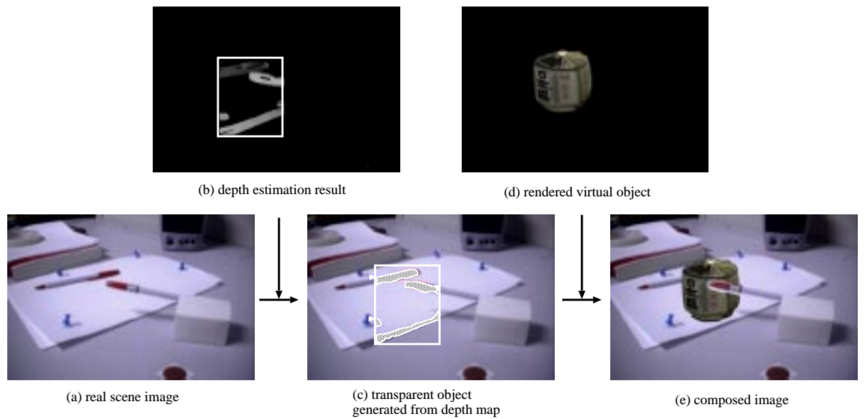
\includegraphics[width=1.0\textwidth]{content/images/methods/stereo-depth-map.png} 
  \caption{Visualisierung des Methode zur Vedeckung durch Depth Maps. Übernommen von \citet{kanbara2000stereoscopic}}
  \label{fig:stereo-depth-map}
\end{figure}

Als Erstes werden in diesem Verfahren 2D Bounding Boxen der zu rendernden virtuellen Objekte auf dem Viewport aus beiden Sichtfeldern der Stereokamera bestimmt. Die 2D Bounding Box wird durch eine Viewport Projektion der 3D Bounding Box eines virtuellen Objektes erzeugt. Diese Bounding Box Regionen wurden zunächst ermittelt, um die Bestimmung von Tiefeninformationen aus Performancegründen auf diese Bereiche zu beschränken. Als nächstes wird in den ermittelten Regionen ein Stereomatching mit Ecken aus der Anwendung des Sobel Filter durchgeführt. Hieraus können darauf folgend Tiefeninformationen der reellen Umgebung gewonnen werden. \citep{kanbara2000stereoscopic} \\

Da die Projekt Tango Hardware direkt Tiefeninformationen durch den Infrarot Laser liefert, wird das Stereomatching hier nicht weiter erläutert. Die Bestimmung von Bounding Boxen, wie von \citet{kanbara2000stereoscopic} beschrieben, ist somit auch nicht für die weitere Anwendung mit Project Tango relevant.\\


Um den Ausschluss der Pixel eines virtuellen Objektes, welches sich hinter einem reellen Objekt befinden, zu verhindern, wird der Z-Buffer Algorithmus nach \citet{greene1993hierarchical} angewendet. Dabei werden zunächst die ermittelten realen Tiefeninformationen in den Z-Buffer gefüllt. Das führt dazu, dass ein virtueller Bildpunkt des zu rendernden Objektes, welcher einen höheren Z-Wert als der bereits vorhandene Wert im Z-Buffer hat, also weiter vom Betrachter entfernt ist, nicht in den Framebuffer gelangt. In Abbildung \ref{fig:stereo-depth-map} ist das Vorgehen dieses Verfahrens noch einmal dargestellt, wobei im Fall von Project Tango Schritt \(b ) \) nicht angewendet wird. \\




\section{Echtzeit Polygon Rekonstruktion} \label{sec:polygon_reconstruction}

Die Idee der Verdeckung mit Hilfe des Z-Buffers lässt sich nicht nur direkten mit Depth Maps aus den Tiefenpunkten realisieren. Auch Primitiven oder allgemein Polygone könnten mit Hilfe eines entsprechenden Fragment Shaders, als Repräsentation der Umgebung, andere virtuelle Objekte Transparent überlagern, um die Illusion der Überdeckung von realen Objekten zu ermöglichen. Somit ließe sich das Problem der Optimierung von Augmented Reality mit Hilfe von Tiefeninformationen auf das Problem der Echtzeit Rekonstruktions zurückführen. \\

Die 3D Rekonstruktion ist bereits ein etabliert Forschungsgebiet in der Computer Grafik und gewinnt, auf Grund von kostengünstigen Consumer Tiefensensoren, wie die Microsoft Kinect, Asus Xtion oder Structure \citep{Struc48:online}, zunehmend an Bedeutung. Dabei wird sich immer mehr auf die Echtzeit Rekonstruktion konzentriert, da diese Geräte in der Lage sind, Tiefeninformationen, zwar mit leichten Messfehlern aber in Echtzeit, zu liefern. \citet{niessner2013real} erwähnen an dieser Stelle zudem den möglichen Einsatz für Augmented Reality:

\begin{quote}
\enquote{The ability to obtain reconstructions
in real-time opens up various interactive applications including:
augmented reality (AR) where real-world geometry can be fused
with 3D graphics and rendered live to the user; ...} \citep{niessner2013real}
\end{quote}

Die Herausforderung in der Echtzeit Rekonstruktion liegt dabei in der möglichst performanten Fusion von mehreren überlagernden Depth Maps. Hieraus soll eine möglichst detailierte Repräsentation der echten Umgebung generiert werden, welche sich im Idealfall stetig verbessert. Diese Problemstellung unterscheidet sich von herkömmlichen Rekonstruktionsverfahren wie die von \citet{hoppe1992surface} und der Poission Rekonstruktion von \citet{kazhdan2006poisson}. Aktuelle Verfahren nutzen dafür verschiedenste optimierte Datenstrukturen, welche zudem durch den Einsatz von entsprechenden GPU Implementierungen beschleunigt werden können. Dennoch spielt die Gegenüberstellung von Detailgrad, der Skalierung und Geschwindigkeit stets eine große Rolle. \citet{niessner2013real} \\

Bekannte Verfahren wie KinectFusion \citep{newcombe2011kinectfusion}, ein SLAM Verfahren von \citet{bylow2013real} oder DynamicFusion \citep{newcombe2015dynamicfusion} nutzen die \enquote{Truncated Signed Distance Function}, kurz TSDF, zur Speicherung und Migration der Oberflächeninformation mehrerer Depth Maps. Das Verfahren von \citet{niessner2013real} erweitert diesen Ansatz mit einem effizienten Spatial Hashing Verfahren, um die Zugriffszeiten und Speicherverbrauch zu minimieren. Darüber hinaus nimmt das Verfahren Chisel von \citep{Klingensmith_2015_7924} diese Vorzüge auf und kombiniert TSDF mit  \enquote{visual-inertial odometry}, der Trackingtechnologie von Project Tango. In den folgenden Absätzen werden die Mechanismen hinter TSDF, dem räumlichen Hashing und den Vorzügen von Chisel näher erläutert. Außerdem soll auch noch auf das Rendering der TSDF Oberfläche durch Marching Cubes eingegangen werden, welches in Chisel verwendet wird. \\


\subsection{Truncated Signed Distance Function}

Bei der von \citet{curless1996volumetric} vorgestellten räumlichen Repräsentation von Oberflächen, Truncated Signed Distance Function (TSDF), wird der Raum in Voxel einer gewünschten Auflösung unterteilt. Anders als Occupancy Maps, in denen die Voxel als sichtbar oder unsichtbar markiert werden, werden bei TSDF in den Voxeln die jeweiligen Entfernungen zur nächsten Oberfläche angegeben. Wichtig dabei ist das Vorzeichen, welches angibt, ob sich ein Voxel innerhalb oder außerhalb eines Objektes befindet. Abbildung \ref{fig:tsdf} zeigt unter a) die Ergebnisse mit Occupancy Maps und in b) die Voxel von TSDF. \citep{curless1996volumetric} \\

Gefüllt wird die Repräsentation durch die Depth Maps und der entsprechenden Kameraposition, die im Fall von Project Tango bereits gegeben ist. So wird für jede Tiefeninformation ein Strahl ausgehend von der Kameraposition generiert, der die durchgeschnittenen Voxel aktualisiert. Der Stahl ist dabei von der Länge begrenzt, um die zu aktualisierenden Voxel zu minimieren und zudem keine Oberflächen zu aktualisieren, die sich weiter hinter der gefundenen Oberfläche befindet. Dieses Vorgehen ist in Abbildung \ref{fig:tsdf} c) zu erkennen. \citep{Compu66:online} \\

\begin{figure}
  \centering
	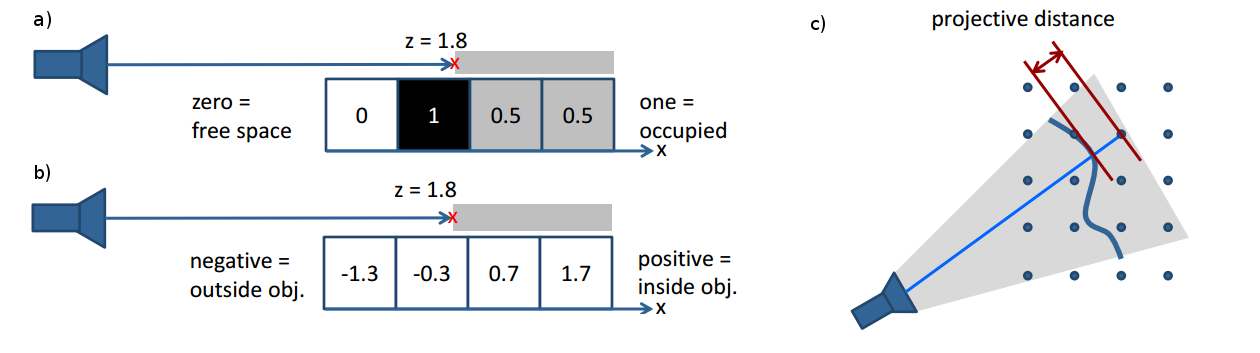
\includegraphics[width=1.0\textwidth]{content/images/methods/tsdf.png} 
  \caption{a) Beispielhafte Voxel Füllung von Occupancy Maps; b) Beispielhafte Voxel Füllung durch TSDF; c) Exemplarische 2D Darstellung der Oberfläche mit entsprechenden Strahlensatz für die TSDF. Übernommen von \citet{Compu66:online}}
  \label{fig:tsdf}
\end{figure}

Der Vorteil dieser Repräsentation liegt darin, dass die konkreten Oberflächeninformationen, anders als bei der Diskretisierung von Occupancy Maps, nicht verloren gehen. Das heißt, dass trotz einer gröberen Voxel Struktur stets der Nulldurchgang rekonstruiert werden kann. Neben der Entfernung zur nächsten Oberfläche wird zusätzlich noch ein Gewichtungswert in jedem Voxel gespeichert. Das ermöglicht es leichtes Rauschen durch einfache Mittelung zu unterdrücken und die Oberfläche optimiert sich somit bei jeder Aktualisierung der Voxel. \citep{Compu66:online}\\

\citet{hoppe1992surface} nutzen in Ihrem Rekonstruktionsverfahren auch die hier beschriebene TSDF. Jedoch bestimmen sie für jeden festgehaltenen Punkt der Pointcloud die umliegenden Nachbarn, um eine Tangentialebene zu ermitteln, von der aus die auf der Normalen liegenden Voxel mit der entsprechenden Distanz aktualisiert werden. Für die Echtzeitrekonstruktion ist dieses Vorgehen jedoch zu komplex. Hier werden die Voxel nicht anhand der exakten euklidischen Distanz aktualisiert, sondern es wird mit Hilfe des Raycastings, ausgehend von der Tiefenkamera, eine projizierte Distanz als Approximation verwendet. \citep{Compu66:online}

\subsection{Spatial Hashing}

Das Problem der Echtzeit Rekonstruktion ist wie bereits angesprochen der Kompromiss zwischen dem Detailgrad, der Skalierung der zu rekonstruierenden Szene und der Performance der Rekonstruktion. Auch die TSDF Repräsentation ist sehr speicherintensiv und benötigt für die zu scannende Szene reservierten Speicher, der auf mobilen Endgeräten nur begrenzt verfügbar ist. Daher muss auch für größere Rekonstruktionen oder Rekonstruktionen unbekannter Größe ein dynamischer Ansatz gefunden werden. \citet{Klingensmith_2015_7924} erwähnt dazu, dass einige Verfahren Octrees einsetzen, die zwar äußerst dynamisch sind, jedoch einen deutlichen Nachteil hinsichtlich der Zugriffszeiten auf die Voxel bergen. \\

\begin{figure}[h]
  \centering
	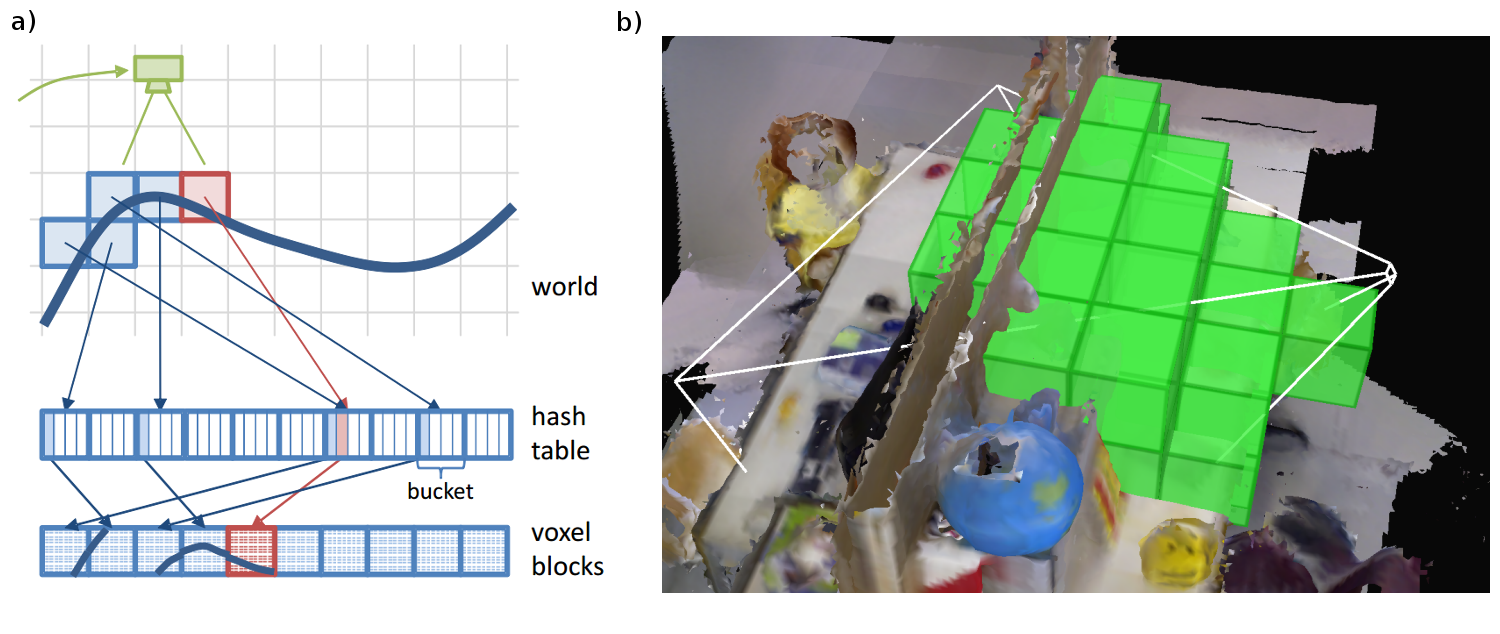
\includegraphics[width=1.0\textwidth]{content/images/methods/hashing.png} 
  \caption{a) Voxel Hashing Datenstruktur. Übernommen von \citet{niessner2013real} b) Darstellung der relevanten Voxel Chunks für die Aktualisierung. Übernommen von \citet{Klingensmith_2015_7924}}
  \label{fig:hashing}
\end{figure}

\citet{niessner2013real} führen daher eine zwei-Ebenen Struktur ein, die auf der zweiten Ebene eine Menge von Voxel räumlich zusammenfassen. Diese werden hier Chunks genannt. Auf der ersten Ebene können diese Chunks in einer Hash Tabelle räumlich mit einer Hashfunktion identifiziert werden. Das ermöglicht somit einen nahezu direkten Zugriff auf räumliche Voxel und ermöglicht es zudem Chunks dynamisch zu allokieren. Als Hash der Chunkposition \(x\), \(y\) und \(z\) wird die folgende Hashfunktion aus Gleichung \ref{eq:spatial_hash} verwendet. Bei den Variablen \(p_1\), \(p_2\) und \(p_3\) handelt es sich um willkürlich hohe Primzahlen und \(n\) entspricht der Größe der Hash Tabelle. 

\begin{equation}\label{eq:spatial_hash}
H(x,y,z) = (x * p_1 \oplus y * p_2 \oplus z * p_3) \mod n
\end{equation}

\subsection{Marching Cubes}

Die meisten Echtzeit Rekonstruktionen durch TSDF wie KinectFusion sind GPU Umsetzungen, die daher die Möglichkeit besitzen ein hardwarebeschleunigtes Rendering durch Raycasting durchzuführen. Das Verfahren Chisel von \citet{Klingensmith_2015_7924}, welches eine reine CPU Umsetzung ist, nutzt hingegen einen indirekten Weg zum Rendering durch die Marching Cubes Triangulation. \\

\begin{figure}[h]
  \centering
	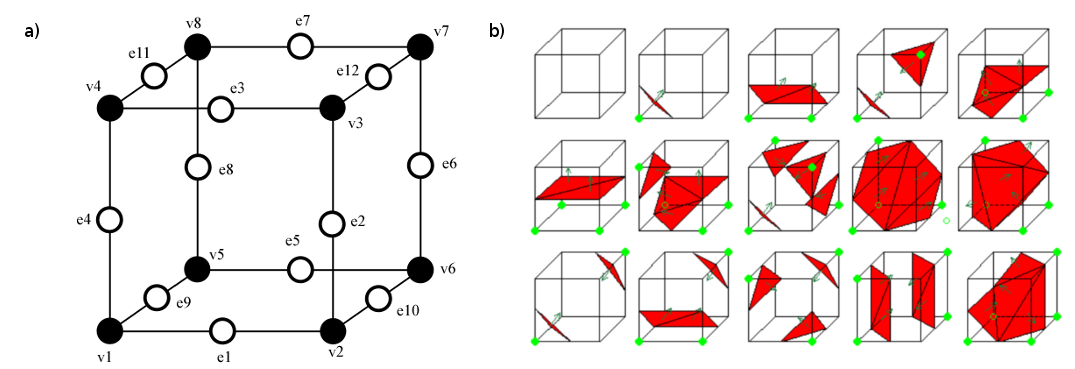
\includegraphics[width=1.0\textwidth]{content/images/methods/marchingcubes.png} 
  \caption{a) Marching Cubes Voxel Repräsentation mit den Ecken und den Kantenschnittpunkten b) Die 15 möglichen 3D Polygon Varianten. Übernommen von \citet{MarchingCubes:online}}
  \label{fig:marchingcubes}
\end{figure}

Marching Cubes nach \citet{lorensen1987marching} ist ein Algorithmus um aus einer, als Voxel repräsentierten, Isofläche Polygone zu bestimmen, die dieser Fläche möglichst nah kommt. Hierzu werden zu jedem Voxel die Ecken \(v1\) bis \(v8\) anhand der Nachbarvoxel und des Distanzwertes untersucht, ob sie innerhalb oder außerhalb eines Objektes liegen. Zusätzlich werden zu jeder Kante auf dem Voxel, wenn ein Schnitt der Isofläche existiert, die Schnittpunkte auf den Kanten \(e1\) bis \(e12\) bestimmt. Abbildung \ref{fig:marchingcubes} a) zeigt die Ecken und Kantenschnittpunkte eines Voxels. \\

Je nach binärer Gewichtung der Ecken können hiernach aus einem Katalog von 256 Varianten die Polygone nachgeschlagen werden. Inhalt des Katalogs sind die Indizes der Kantenschnittpunkte, aus denen Polygone generiert werden können. Alle diese 256 Varianten können auf 15 verschiedene Fälle zurückgeführt werden, die sich nur in Rotation oder Symmetrie unterscheiden. Die 15 Varianten sind in Abbildung \ref{fig:marchingcubes} b) zu finden. \citep{MarchingCubes:online} \\

\subsection{Chisel mit Space Carving}

Das Bereits erwähnte Verfahren Chisel von \citet{Klingensmith_2015_7924} verwendet alle zuvor erwähnten Techniken der TSDF, spatial Hashing und der Marching Cubes Überführung. Sie sprechen dabei von einem \enquote{dynamic spatial-hashed truncated distance field}. Das für den mobilen Einsatz optimierte Verfahren ist in der Lage eine Echtzeitrekonstruktion von Räumen von bis zu \(300 m^2\) mit einem Detailgrad von zwei bis drei Zentimetern zu erstellen. Zudem können neben Tiefeninformationen auch gefärbte Pointclouds verarbeitet werden, wodurch ein gefärbtes Mesh generiert werden kann. \citep{Klingensmith_2015_7924}\\

Zusätzlich erweitern sie den TSDF Algorithmus um die \enquote{space carving} Funktionalität. Sie betrachten dabei den Strahl von der Kamera zur Oberfläche als eine Art Constraint, in dem alle durchstoßenden Voxel bis zur Oberfläche eine negativen Wert beinhalten müssen. Ist das nicht der Fall, so wird ein Voxel außerhalb der inneren Begrenzung auf den leeren Ursprungswert gesetzt. Im Pseudocode aus Listing \ref{lst:chisel} wird das Verhalten näher erläutert. Diese Verbesserung führt dazu, dass die Rekonstruktion bei stark rauschenden Tiefeninformationen, besonders an Objektkanten, deutlich verbessert wird. Außerdem ist das Verfahren hiermit in der Lage dynamische Änderungen in der Umgebung zu detektieren und neue Oberflächen entsprechend zu aktualisieren. So beeinflussen zum Beispiel sich im Bild bewegen Personen nur kurz die Voxel der TSDF. \citep{Klingensmith_2015_7924}\\

\begin{lstlisting}[mathescape,caption=Chisel TSDF Algorithmus, label=lst:chisel]
Eingabe: Pointcloud $C$, Kameratransformation $P_{cam}$, 
         Strahlenbegrenzung $t$

für jeden Tiefenwert $\vec{p}$ aus $C$
    bestimme die Oberflächenposition $\vec{z}$ aus $\vec{p}$ und $P_{cam}$
    bestimme einen Strahl $\vec{r}$ aus $\vec{z}$ und $P_{cam}$
    bestimme den Begrenzungsbereich $t_{vor}$, $t_{nach}$ mit $t$ um $\vec{z}$ auf $\vec{r}$
    # space carving
    für jeden Voxel $v$ zwischen Kamera und $t_{vor}$
        wenn die Distanz im Voxel negativ ist
            setze Voxel zurück
    # normale TSDF Bestimmung
    für jeden Voxel $v$ zwischen $t_{vor}$ und $t_{nach}$
        bestimme die Voxeldistanz zu $z$
        setze das Gewicht w des Voxels $v$
\end{lstlisting}

Neben space carving wurden zudem eine variable Strahlenbegrenzungen und Gewichtungen der Voxel abhänig von der jeweils aufgenommenen Tiefe implementiert. Diese Funktion berücksichtigt die Varianzen von Messungenauigkeiten des Sensors, die bei größerer Entfernung der Oberfläche zum Tiefensonsor zunehmen können. \citep{Klingensmith_2015_7924}

\textbf{TODO:} DARSTELLUNG DES STRAHLS, DER KAMERA UND DER OBERFLÄCHE ZUR VERSTÄNDNIS DES ALGORITHMUS

\section{Planare Rekonstruktion} \label{sec:plane-reconstruction}

Dieses Kapitel widmet sich der Idee, eine Rekonstruktion für ein Rekonstruktions basiertes Überlagerungsverfahren durch eine Ebenendetektion zu realisieren. \citet{yang2010plane} erwähnt hierzu, dass Ebenen in fast allen künstlichen Umgebungen zu finden sind und auf Grund ihrer vorteilhaften geometrischen Eingenschaften in verschiedensten Computer Vision Verfahren verwendet werden. Daher gibt es viele Forschungsarbeiten, Methoden und Algorithmen, um aus verschiedensten Informationsquellen ein Ebenenmodell zu extrahieren.\\

Das \enquote{Simultaneous Localization and Mapping} (SLAM) Verfahren von \citet{trevor2012planar} detektiert Ebenen mit dem RANSAC Algorithmus. RANSAC bietet gegenüber anderen Algorithmen zur Ebenen Detektion den Vorteil, ein Modell auch bei vielen Ausreißern performant zu ermitteln. Agglomeratives Clustering und Region Growing wie von \citet{feng2014fast} beschreiben, eignet sich auf Grund des Ausgabeformats von Project Tango nicht direkt, da es keine organisierte Point Cloud ausgibt und die Daten durch Reflektionen und Löchern mit Fehlern behaftet sind. \\

Das selbst zusammengestellte Verfahren zur Ebenendetektion besteht daher aus folgenden Komponenten. Wie in dem Ansatz von \citet{yang2010plane} wird der RANSAC Algorithmus auf Würfeln ausgeführt, die eine Menge gesammelter Punkte aus der Pointcloud beinhaltet. Dabei entsprechen die Würfel den untersten Knoten eines Octrees, welcher hier zur Speicherung und Aufnahme aller Punkte verwendet wird. Eine gefundene Ebene in einem Würfel wird wie im SLAM Verfahren von \citet{trevor2012planar} persistiert. Die Repräsentation der Ebene \(P\) wird dort wie in Gleichung \ref{eq:plane} festgehalten. Dabei handelt es sich um den Normalenvektor \(\vec{n}\) und der Distanz zum Ursprung \(d\) der Hesse Normalform einer Ebene, sowie der Punkte der konvexen Hülle \(H\). \citet{trevor2012planar} erläutern, dass die konvexe Hülle in der Repräsentation festgehalten wird, um eine sukzessive Verbesserung einer Ebene nach mehreren Messdurchläufen zu ermöglichen. So werden die Punkte der konvexen Hülle pro Messvorgang kombiniert, damit die Ebenenausbreitung auch außerhalb des Sichtfeldes beibehalten werden kann. \\

\begin{equation} \label{eq:plane}
P=\left[\vec{n}, d, H\right] \qquad H=\vec{h_1}, \vec{h_2}, \ldots  \vec{h_n}
\end{equation}

Die einzelnen Schritte des Vorgehens werden in den folgenden Absätzen näher erläutert. Ein grober Ablauf des Vorgehens wird aber bereits in Listing \ref{lst:planeReconstruction} zusammengefasst und in Pseudocode beschreiben. Als Cluster sind im Listing sind die untersten Nodes eines Octrees gemeint.

\begin{lstlisting}[mathescape,caption=Planare Echtzeit Rekonstruktion, label=lst:planeReconstruction, float=htbp]

Eingabe: Octree $O$, Anzahl der zu suchenden Ebene in Clustern $N$
Ausgabe: Polygonpunkte $T_{Gesamt}$

für jedes Cluster $C$=[$C_{Punkte}$, $C_{Ebenen}$] aus $O$
    führe $N$ mal aus
        bestimme Ebene [$\vec{n}$, $d$, $P$] mit RANSAC aus $C_{Punkte}$
        wenn keine Ebene mit genügend $P$ gefunden wurde
            nächstes Cluster (continue)
        wenn Ebene mit [$\vec{n}$, $d$, $H_{alt}$] in $C_{Ebenen}$ existiert	
            füge die konvexe Hülle $H_{alt}$ zu $P$ hinzu	
        bestimme die konvexe Hülle $H_{neu}$
        trianguliere $H_{neu}$ zu $T_{Ebene}$
        $T_{Gesamt}$ += $T_{Ebene}$
        $C_{Ebenen}$ += [$\vec{n}$, $d$, $H_{neu}$]
        $C_{Punkte}$ - $P$
\end{lstlisting}


\subsection{RANSAC zur Ebenendetektion} \label{sec:ransac}

Um mit dem RANSAC Algorithmus, beschrieben in Kapitel \ref{sec:ransac-theory}, Ebenen in einer Punktewolke bestimmen zu können, werden pro Iteration drei Stichproben \(\vec{A}\), \(\vec{B}\) und \(\vec{C}\) gewählt, die zur Bestimmung einer Ebene ausreichen. Das Ebenenmodell, hier in der Hesse Normalform mit dem Normalenvektor \(\vec{n}\) und dem Abstand zum Koordinatenursprung \(d\), lässt sich dabei durch die Gleichung \ref{eq:normalform} bestimmen.

\begin{equation}\label{eq:normalform}
\vec{n} =\left|\left| \vec{AB} \times \vec{AC}\right|\right|
\qquad
d = \vec{A} \cdot \vec{n}
\end{equation}

Um zu ermitteln ob ein Punkt \(\vec{P}\) aus einer Messreihe die gefundene Ebene \(\left[\vec{n}, d\right]\) unterstützt, wird die kürzeste Distanz \(d_P\) zwischen Punkt und Ebene wie in Gleichung \ref{eq:plane-distance} ermittelt.  Ein entsprechender Toleranzwert für die Distanz \(d_{min}\), im gezeigten RANSAC Algorithmus \(e\) genannt, wird später bei der Umsetzung abhängig von der Ungenauigkeit des Tiefensensors gewählt. 

\begin{equation} \label{eq:plane-distance}
d_P = \vec{n} \cdot \vec{P} - d \qquad support_{d_P} = d_P < d_{min}
\end{equation}

Um das finale Modell der Ebene zu ermitteln, wie im Ursprünglichen RANSAC Algorithmus in Punkt 7. beschrieben, und somit die Varianz des Abstands der Punkte zur Ebene zu minimieren, wird mit Hilfe der unterstützenden Punkte \(P_{s}=\left[x,y,z\right]\) eine lineare Regression durchgeführt. Diese Mittelt ein Ebenenmodell \(E=\left[\vec{n}, d\right]\) aus den zuvor ermittelten Punkten mit Hilfe der Methode der kleinsten Quadrate. \citet{hoppe1992surface} nutzen hierfür für eine ähnliche Problemstellung die Eigenwert Dekomposition der Kovarianzmatrix der Punkte \(P_{s}\) zum Zentrum \(\vec{p_{c}}\). In Gleichung \ref{eq:centroid} wird das Zentrum aus den unterstützenden Punkten \(P_{s}\) bestimmt. Gleichung \ref{eq:covarianz} zeigt die Bestimmung der Kovarianzmatrix \(CV\) im Bezug zum Zentroid, in der \(\otimes\) für das dyadische Produkt\footnote{Wenn \(\vec{a}\) und \(\vec{b}\) die Komponenten \(a_i\) und \(b_j\) beinhalten, resultiert aus \(\vec{a} \otimes \vec{b}\) eine Matrix mit den Komponenten \(a_ib_j\) an der \(ij\) Position. \citep{hoppe1992surface}} steht.

\begin{equation} \label{eq:centroid}
\vec{p_{c}} = \frac{\sum_{n=0}^{|P|} P_{n}}{|P|}
\end{equation}

\begin{equation} \label{eq:covarianz}
CV = \sum_{n=0}^{|P|} ( \vec{p_{n}}- \vec{p_{c}}) \otimes ( \vec{p_{n}}- \vec{p_{c}})
\end{equation}

Wendet man nun auf der Kovarianzmatrix \(CV\) die Eigenwert Dekomposition an, erhält man die Normale \(\vec{n}\) aus dem Eigenvektor \(||\vec{v_i}||\) mit dem kleinsten Eigenwert \(\lambda_i\). Somit würde bei \(\lambda_1 \geqq \lambda_2 \geqq \lambda_3\) die Zuweisung \(\vec{n} = ||\vec{v_3}||\) folgen. Die Distanz zum Ursprung \(d\) entspricht dem Kreuzprodukt aus dem Zentroiden \(\vec{p_c}\) und der neu gewonnen Normalen \(\vec{n}\). \citep{hoppe1992surface} \\

\subsection{Bestimmung der Ebenenausbreitung}

Nachdem die Ebene und die korrespondierenden Punkte zur Ebene gefunden wurden, muss noch die Ausbreitung der Fläche bestimmt werden, da die Ebene in Hesse Normalform lediglich die Position \(\vec{n} * d\) und Ausrichtung \(\vec{n}\) festhält. \citet{PlanarSurfaceMapping} nutzt hierfür die konvexe Hülle der korrespondierenden Punkte und trianguliert diese. Wie diese dort genau bestimmt wurde ist nicht beschrieben. \\

Um diese Bestimmung performant umsetzen zu können, kann man sich hier die Eigenschaft der Ebene zu Nutzen machen und die dreidimensionalen Punkte durch Parallelprojektion als zweidimensionale Punkte auf die Ebene projizieren. Denn die Triangulation ist nach dem Erhalten der zweidimensionalen konvexen Hülle, wie im Listing \ref{lst:triangulation} beschrieben, direkt bestimmbar. Nach der Triangulation können die Ecken der gefundenen Polygone jeweils zurück projiziert werden. Die Gleichungen \ref{eq:projection2d} und \ref{eq:projection3d} bilden die Projektion der Punkte wobei \(R_{\vec{n} \rightarrow \vec{z}}\) der Rotationsmatrix zwischen dem Normalenvektor \(\vec{n}\) und der Z-Achse \(\vec{z}\) entspricht.\\

\begin{equation} \label{eq:projection2d}
p_{2d} = (p_{3d} - (\vec{n}*d)) * R_{\vec{n} \rightarrow \vec{z}}
\end{equation}
\begin{equation} \label{eq:projection3d}
p_{3d} = (p_{2d} * R_{\vec{n} \rightarrow \vec{z}}^{-1}) + (\vec{n}*d)
\end{equation}

\begin{lstlisting}[mathescape,caption=Bestimmung der Ebenenausbreitung und Triangulation, label=lst:triangulation, float=htbp]

Eingabe: Unterstützende Ebenenpunkte aus RANSAC $P$
         Transformation $R_{\vec{n} \rightarrow \vec{z}}$
Ausgabe: Polygone $T_{Ebene}$

    Projiziere alle Punkte aus $P_s$ mit $R_{\vec{n} \rightarrow \vec{z}}$ zu $P_{2d}$
    Bestimme die konvexe Hülle $H$ aus $P_{2d}$ mit Graham Scan
    starte mit leerer Menge $P_{2dmesh}$
    für $i$ von $0$ bis $|H| - 2$
        füge $H_i$ zu $P_{2dmesh}$ hinzu
        füge $H_{i+1}$ zu $P_{2dmesh}$ hinzu
        füge $H_{i+2}$ zu $P_{2dmesh}$ hinzu
    Projiziere alle Punkte aus $P_{2dmesh}$ mit $R_{\vec{n} \rightarrow \vec{z}}^{-1}$ zu $P_{3dmesh}$
   
\end{lstlisting}


\subsection{Clustering der aufgenommenen Punkte} \label{sec:cluster}

Wie im Listing \ref{lst:planeReconstruction} zu erkennen wird das zuvor beschriebene Vorgehen für die planare Rekonstruktion immer pro Cluster eines Cluster-Pools durchgeführt. Dadurch werden pro Durchgang des Algorithmus nur ein Bruchteil der gesammelten Punkte rekonstruiert, was wiederum eine Rekonstruktion in Echtzeit möglich macht. Außerdem verhindert das Clustering das Bilden von konvexen Hüllen über Ebenen, die in Zwischenbereichen nicht mit genügend Punkten unterstützt werden. Dieses Problem ist in Abbildung \ref{fig:clustering} links zu sehen, in welcher eine blaue Ebene Rekonstruiert wird, die sich über einen Durchgang ohne vorhandene Punkte streckt.\\

\begin{figure}[h]
  \centering
	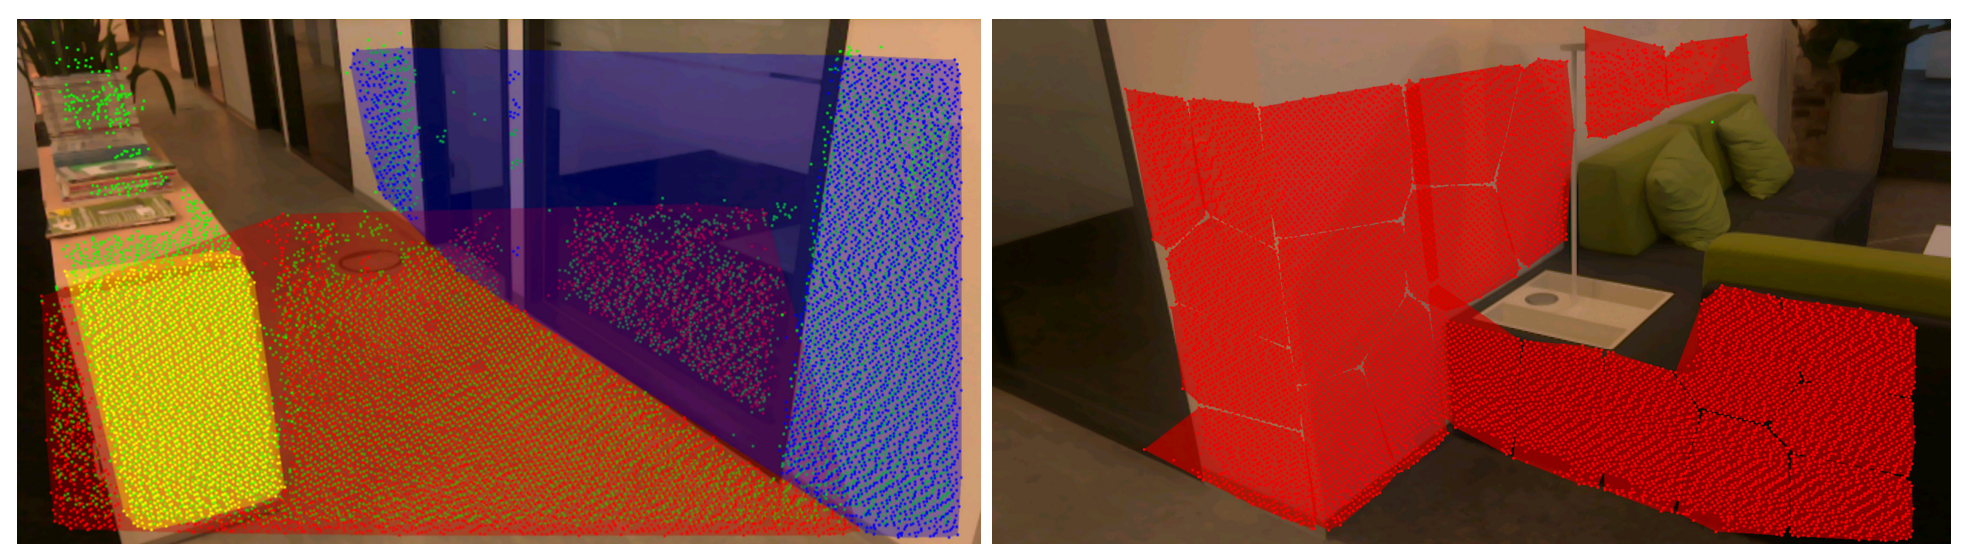
\includegraphics[width=1.0\textwidth]{content/images/methods/clustering.png} 
  \caption{Links: Ebenenrekonstruktion ohne Clustering. Rechts: Rekonstruktion mit K-Mean Clustering.}
  \label{fig:clustering}
\end{figure}

Getestet wurden hier das K-Mean Clustering, Agglomeratives Clustering und einfaches räumliches Clustern mit Hilfe eines Octrees. Das K-Mean Clustering hat, wie in Abbildung \ref{fig:clustering} rechts zu erkennen, gute Ergebnisse für die Aufteilung einer Ebenen geliefert, benötigt aber zuvor eine feste Anzahl von Clustern. Agglomeratives Clustering, getestet mit dem euklidischen Distanzmaß, würde zwar die Anzahl der Cluster dynamisch bestimmen, ist jedoch zu aufwändig für eine Echtzeit Rekonstruktion. \\

Gute Ergebnisse liefert wiederum ein einfaches räumliches Clustern mit einem Octree, welcher die aufgenommenen Punkte direkt in Knoten des Baums zuweist. Das bietet zudem den Vorteil, dass diese Datenstruktur direkt als Speicherort der Aufgenommenen Punkte und Ebenen dienen kann. Außerdem entspricht dies dem Vorgehen für die Anwendung von RANSAC auf Würfeln, welches von \citet{yang2010plane} beschrieben wurde. \\


\section{Tiefenanpassungen durch Farbbilder}

Aus allen zuvor beschriebenen Verfahren werden letztendlich Tiefeninformationen, in Form von geometrischen Primitiven oder Punkten im Raum gewonnen. Diese werden passend zur aktuellen Kameraposition als Tiefenbild gerendert und füllen den Z-Buffer für eine entsprechende Aussparungen bei der Überdeckung virtueller Objekte. Auf Grund von Sensorungenauigkeiten und den daraus resultierenden größeren Auflösungen der Rekonstruktionsverfahren können dabei fehlerhafte Tiefeninformationen im Z-Buffer gelangen, die zu Fehlern bei der Bestimmung der Überdeckung führen können. Dieses Problem ist am Beispiel der Pointcloud Projektion aus Kapitel \ref{sec:pc-projection} in Abbildung \ref{fig:pc-noise} zu erkennen. \\

\begin{figure}[h]
  \centering
	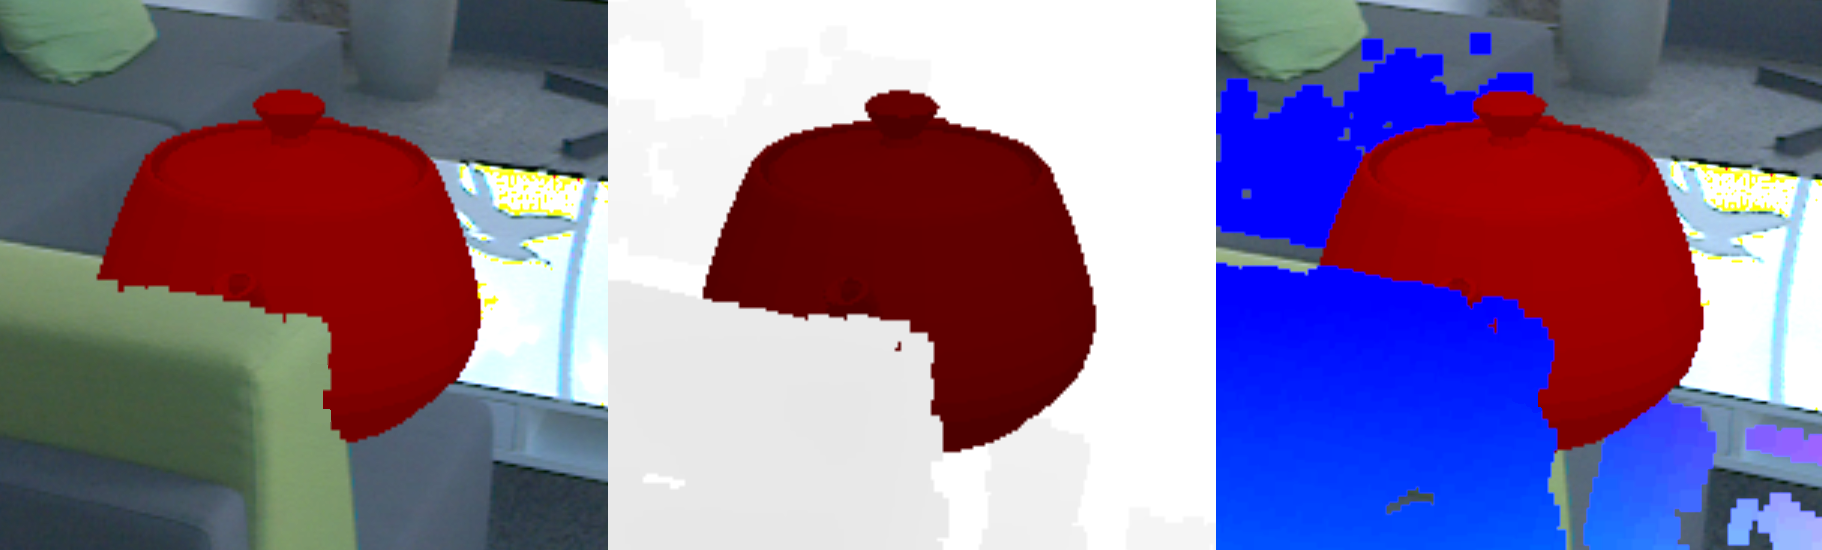
\includegraphics[width=1.0\textwidth]{content/images/methods/pc-noise.png} 
  \caption{Überdeckung mit einfacher Pointcloud Projektion. Links: Resultat der Überdeckung. Mitte: Darstellung des Tiefepuffers. Rechts: Darstellung der Pointcloud.}
  \label{fig:pc-noise}
\end{figure}

Die Reduktion von Ungenauigkeiten im Tiefenbild könnte durch einen Gaußschen Weichzeichner erreicht werden. Dieser würde jedoch die Kanten im Farbbild nicht berücksichtigen und somit fehlerhafte Tiefen Gradienten an den Kanten erzeugen. \citet{newcombe2011kinectfusion} wenden einen sogenannten \enquote{Bilateralen Filter} in ihrem KinectFusion System an, bevor sie die Tiefeninformationen in die TSDF Repräsentation einfließen lassen. Dieser Filter von \citet{tomasi1998bilateral} ermöglicht das Weichzeichnen ohne dabei die Kanten im Bild zu übergehen, bezieht sich jedoch nur auf das selbe Bild, auf dem der Filter angewendet wird. \\

\citet{liu2012guided} hingegen wenden einen sogenannten \enquote{Guided Filter} in Ihrem Verfahren zur Optimierung der der Tiefeninformationen für Kinect ähnliche Sensoren auf das Tiefenbild an. Dieser Filter von \citet{he2010guided} ist in der Lage, auf Grundlage eines anderen Leitbildes ein Weichzeichnen durchzuführen, ohne dabei die Kanten des Leitbildes zu überschreiten. Auch wenn \citet{petschnigg2004digital} eine Erweiterung, den Joint Bilateral Filter, vorstellen, der auf Basis eines Leitbildes eine Weichzeichnung ohne Kantenüberschreitung ermöglicht, bietet der Guided Filter eine deutlich bessere Performance. Außerdem verhindert der Guided Filter Fehler Artefakte im Resultat, die bei dem Bilateralen Filter an den Kanten auftreten können. \citep{he2010guided}

\section{Interaktion mit Tiefeninformationen durch Raypicking} \label{sec:ar-depth-interaction}

Wie in Kapitel \ref{sec:ar-interaction} beschrieben, bedarf es bei der Umsetzung von Augmented Reality Systemen ein anderes Interaktionsparadigma. Auch wenn die Entwicklung der neuen Tablet und Smartphone Geräte durch Touchscreens eine neue Interaktionsform eingeführt haben, ist sie in den meisten Fällen auf einer zweidimensionalen Ebene beschränkt. In der Entwicklung von Virtual Reality oder voll virtuellen Anwendungen und Spielen wird oft für die Auswahlgeste der Raypicking Mechanismus verwendet, um eine zweidimensionale Interaktion im dreidimensionalen Raum zu ermöglichen. Darüber hinaus gibt es verbesserte semantische Interaktionsformen basierend auf einer zweidimensionalen Toucheingabe, wie von \citet{elmqvist2008semantic} beschrieben.\\

Hier soll aber zunächst eine Raycasting Variante für Augmented Reality Anwendungen umgesetzt werden, die nicht von einem kompletten Modell in Form von Polygonen oder anderen Primitiven der realen Umgebung ausgeht. Diese AR Interaktionsmöglichkeit ermöglicht, anhand der Tiefeninformationen, das passende Positionieren von virtuellen Objekten im realen Raum und lässt sich auf weitere Interaktionen erweitern. Voraussetzung für die folgende Umsetzung, ist die entsprechende Kalibrierung und Gleichstellung der extrinsischen und intrinsischen Kameraparametern der virtuellen sowie der realen Kamera. \\

\begin{figure}[h]
  \centering
	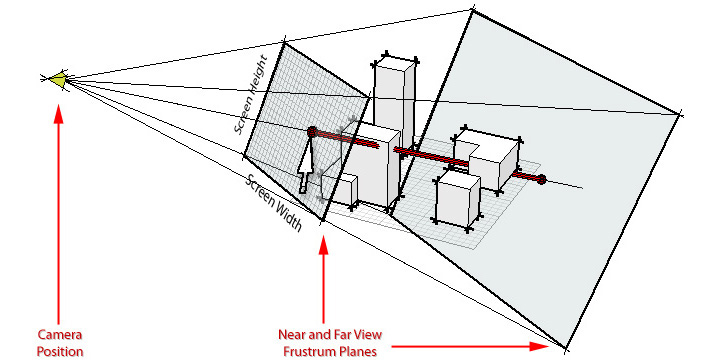
\includegraphics[width=1.0\textwidth]{content/images/methods/interaction.jpg} 
  \caption{Raypicking Visualisierung. Übernommen von \citet{gluUn11:online}}
  \label{fig:interaction}
\end{figure}

Als Erstes wird ein Strahl erzeugt, der durch die Position der virtuellen Kamera und durch den jeweils ausgewählten Punkt auf der Viewingplane läuft. Den Ursprung der virtuellen Kamera bestimmt dabei Google Tangos \enquote{Motion Tracking}. Der gewählte beziehungsweise berührte Punkt auf dem Touchscreen wird dabei zunächst von Pixeln in das Verhältnis \(\left[-1,1\right]\) des Punktes umgerechnet. Hiernach wird die Projektion auf die Viewingplane durch eine Multiplikation mit \(T\) aus Gleichung \ref{eq:unprojection} rückgängig gemacht. Der Gerade aus den beiden Punkten kann danach genutzt werden, um den Schnitt von Objekten vor der Kamera zu ermitteln. \citep{OpenG86:online} 

\begin{equation} \label{eq:unprojection}
T  = MV_{ModelView}^{-1} * P_{Projection}^{-1}
\end{equation}

Angewendet auf die Tiefeninformation aus Tangos \enquote{Depth Perception} wird die Punktewolke, wie in Abbildung \ref{fig:interaction}, vor die Kamera projiziert. In den projizierten Punkten wird danach der entsprechende Punkt gesucht, welcher sich am nächsten am zuvor bestimmten Strahl befindet. Durch diese beschriebenen Schritte kann der Nutzer mit einer zweidimensionalen Geste einen Punkt in der Tiefe bestimmen.

